\documentclass[zihao=-4]{ctexart} % 全局字号设为小四号

% ========== 基本宏包 ==========
\usepackage{xeCJK} % 支持中文
\usepackage{setspace} % 设置行距
\usepackage{multirow} % 支持表格单元格跨行
\usepackage{titlesec} % 自定义标题格式
\usepackage{fancyhdr} % 自定义页眉页脚
\usepackage{indentfirst} % 让第一段也有首行缩进
\usepackage[a4paper, margin=1in]{geometry} % 设置页面布局
\usepackage{lipsum} % 生成示例文本(可移除)
\usepackage[colorlinks=true, linkcolor=black, anchorcolor=blue, citecolor=blue]{hyperref} % 生成 PDF 书签
\usepackage{graphicx} % 支持图形和表格调整
\usepackage{array} % 支持表格列格式调整
\usepackage{amsmath} % 支持数学公式对齐
\usepackage{physics} % 物理符号宏包
\usepackage{siunitx} % 单位符号宏包
\usepackage{tabularray} % 表格宏包
% 设置段首缩进
\setlength{\parindent}{2em} % 设置段首缩进为 2 个字符宽度

% ========== 字体配置 ==========
\setCJKmainfont{SimSun}[ % 全局中文字体为宋体
   BoldFont = SimSun,   % 中文粗体用宋体
   ItalicFont = KaiTi,   % 中文斜体用楷体
   Scale=1.0             % 确保字体大小与字号匹配
]
\setmainfont{Times New Roman} % 英文字体为 Times New Roman
%自定义宋体加粗命令
\newcommand{\boldSun}{\CJKfontspec[FakeBold=3]{SimSun}}

% ========== 行距配置 ==========
\setstretch{1.25} % 设置正文行距为 1.25 倍

% ========== 标题格式 ==========
% 一级标题格式:三号宋体加粗,带中文编号
\titleformat{\section}
  {\zihao{-3}\boldSun} % 标题字体为宋体,模拟加粗
  {\chinese{section}、} % 标题编号格式:X、
  {0.5em} % 编号与标题内容的间距
  {} % 标题前缀

% 二级标题格式:四号宋体加粗
\titleformat{\subsection}
  {\zihao{4}\boldSun} % 标题字体为宋体,模拟加粗
  {} % 不显示编号
  {0em} % 编号与标题内容的间距
  {}
%三级标题格式:小四号宋体
\titleformat{\subsubsection}
    {\zihao{-4}\boldSun} % 小四号字体
    {} % 不显示编号
    {0em} % 编号与标题内容的间距
    {}

% 标题间距设置
\titlespacing*{\section}
  {0pt} % 左缩进
  {0.3\baselineskip} % 上方间距
  {0.3\baselineskip} % 下方间距

\titlespacing*{\subsection}
    {5pt}
    {0.3\baselineskip}
    {0.3\baselineskip}
\titlespacing*{\subsubsection}
    {7.5pt}
    {0.3\baselineskip}
    {0.3\baselineskip}
% ========== 页眉页脚 ==========
\pagestyle{fancy}
\fancyhf{} % 清空默认页眉页脚
\fancyhead{} % 确保页眉清空
\fancyfoot{} % 确保页脚清空
\fancyfoot[C]{\thepage} % 页脚居中显示页码
\renewcommand{\headrulewidth}{0pt} % 去掉页眉下划线
\renewcommand{\footrulewidth}{0pt} % 去掉页脚上划线

% ========== 自定义标题 ==========
\title{实验五\quad 时序逻辑电路}
\author{JS124620\quad 高越}
\date{\today} % 使用当前日期
\makeatletter
% 修改 \@title 的行为
\renewcommand{\maketitle}{
    \begin{center}
        {\zihao{2}\CJKfontspec[FakeBold=3]{SimSun} \@title} \\[0.75em] % 标题为二号宋体加粗
        {\zihao{-4} \@author} \\[0.5em] % 作者为 large 字号
        {\zihao{-4} \@date} % 日期为 small 字号
    \end{center}
}
\makeatother

\begin{document}\zihao{-4}
\maketitle % 显式设置正文为小四号

\section{实验内容} % 自动编号
分别用MSI计数器和移位寄存器设计一个具有自启动功能的010110序列信号发生器
\begin{enumerate}
  \item 写出设计过程,画出电路逻辑图
  \item 搭接电路,并用单脉冲静态验证实验结果 
  \item 加入TTL连续脉冲,用示波器观察观察并记录时钟脉冲CLK、序列输出端的波形。
\end{enumerate}
\section{实验设计方案}
\subsection{方案一\quad 使用MSI计数器的设计方案}
\subsubsection{设计思路}
010110序列信号发生器一个周期内有6个状态,所以应该先用74HC161模16计数器来实现一个模6计数器,
再将该计数器的输出端接入一个组合逻辑电路,从而得到需要的序列。为了使电路简化,可以使用一个3-8译码器来把计数器输出转化为
题目要求的序列,使用同步置数法实现模6计数器。为了进一步简化电路,可以在设计模6计数器时,将74HC138的$\mathrm{\overline{Y5}}$输出端接入74HC161的$\mathrm{\overline{SPE}}$端,实现同步置数,这样可以省去一个非门。
\subsubsection{逻辑电路图}
利用MultiSim软件绘制电路图,电路图如图\ref{fig:161}所示:
\begin{figure}[htbp!]
    \centering
    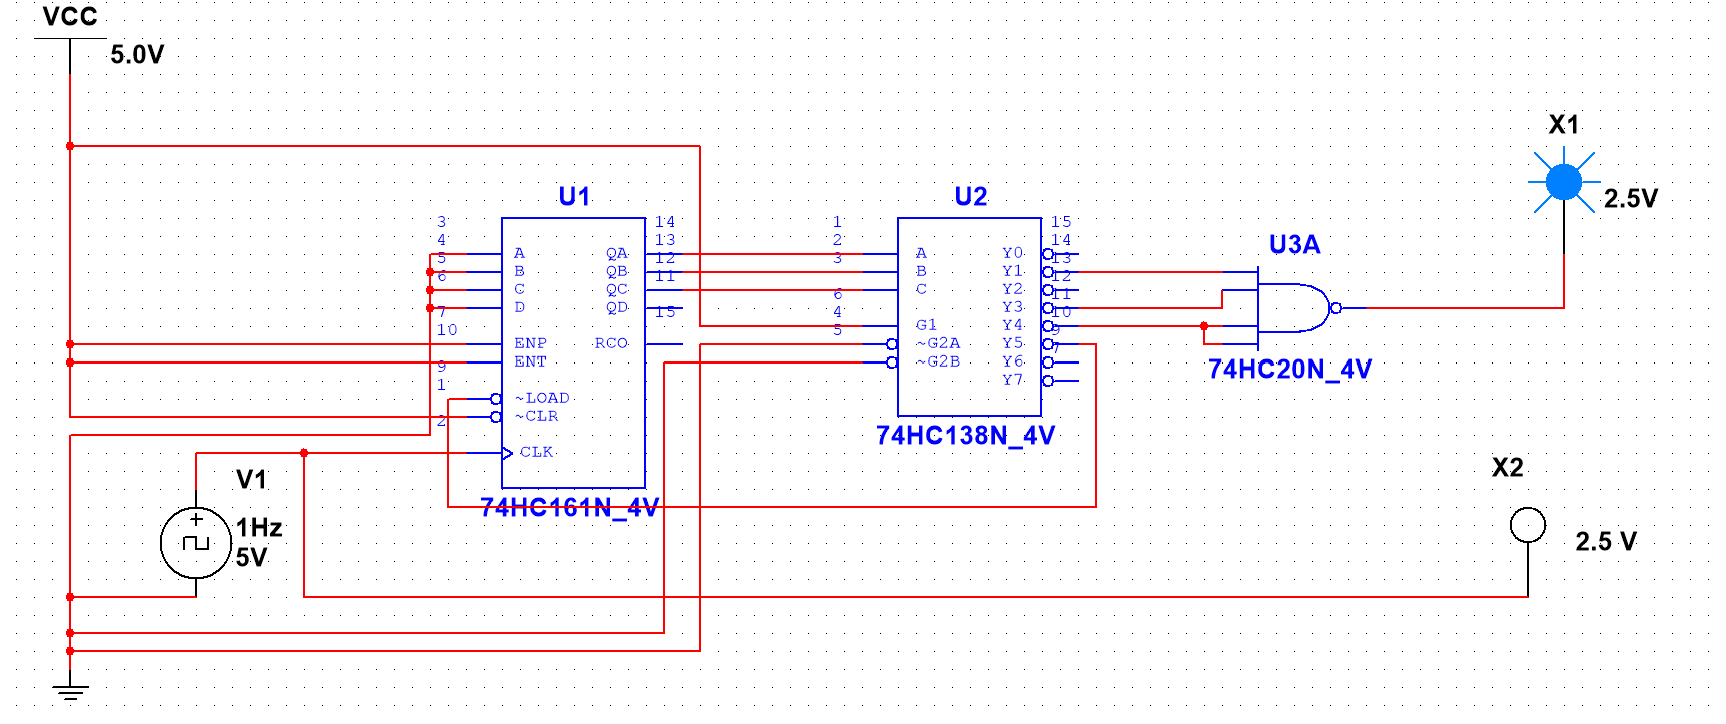
\includegraphics[width=0.8\textwidth]{../img/Ex2_161.png} % 确保文件名和路径正确
    \caption{方案一逻辑电路图}
    \label{fig:161}
  \end{figure}
\subsection{方案二\quad 使用移位寄存器的设计方案}
\subsubsection{设计思路} 
不妨以4位双向移位寄存器的最低输出位$\mathrm{Q_0}$作为输出信号。由于题目要求信号的一个周期内有6个状态,
所以只需用到移位寄存器输出端的最低三位,使用同步置数法来循环产生6个不同状态。因此,只需把$\overline{\mathrm{MR}}$接高电平,四个置数输入端均接地,根据现态控制$S_1$即可。考虑自启动,列出状态转移真值表,如表\ref{tab:state_table} 所示。
% Please add the following required packages to your document preamble:
% \usepackage{multirow}
\begin{table}[]
  \centering
  \begin{tblr}{|c|*{8}{Q[c,m,2.5em]|}}
  \hline
  \SetCell[r=2]{c}   
   & \SetCell[c=3]{c}现态    &  & 
                  & \SetCell[c=3]{c}次态 &  & 
                            & \SetCell[c=2]{c} 控制端 &               \\ 
                            \hline
                          & $\mathrm{Q_2^n}$ & $\mathrm{Q_1^n}$ & $\mathrm{Q_0^n}$ & $\mathrm{Q_2^{n+1}}$ & $\mathrm{Q_1^{n+1}}$ & $\mathrm{Q_0^{n+1}}$ & $\mathrm{D_{SR}}$ & $\mathrm{S_1}$ \\ \hline
  \SetCell[r=6]{c}{有效状态} & 0       & 0       & 0       & 0           & 0           & 1           & 1        & 0     \\ \hline
                          & 0       & 0       & 1       & 0           & 1           & 0           & 0        & 0     \\ \hline
                          & 0       & 1       & 0       & 1           & 0           & 1           & 1        & 0     \\ \hline
                          & 1       & 0       & 1       & 0           & 1           & 1           & 1        & 0     \\ \hline
                          & 0       & 1       & 1       & 1           & 1           & 0           & 0        & 0     \\ \hline
                          & 1       & 1       & 0       & 0           & 0           & 0           & 1        & 1     \\ \hline
  \SetCell[r=2]{c}{无效状态} & 1       & 0       & 0       & 0           & 0           & 0           & 0        & 0     \\ \hline
                          & 1       & 1       & 1       & 0           & 0           & 0           & 0        & 1     \\ \hline
  \end{tblr}
  \caption{方案二状态转移真值表}
  \label{tab:state_table}
  \end{table}
  \subsubsection{逻辑电路图}
  $\mathrm{D_{SR}}$可用数据选择器产生,而从真值表容易看出$\mathrm{S_1=Q_1Q_2}$,故$\mathrm{S_1}$可用与非门实现。
  利用MultiSim软件绘制电路图,电路图如图\ref{fig:SR}所示。
\begin{figure}[htbp!]
    \centering
    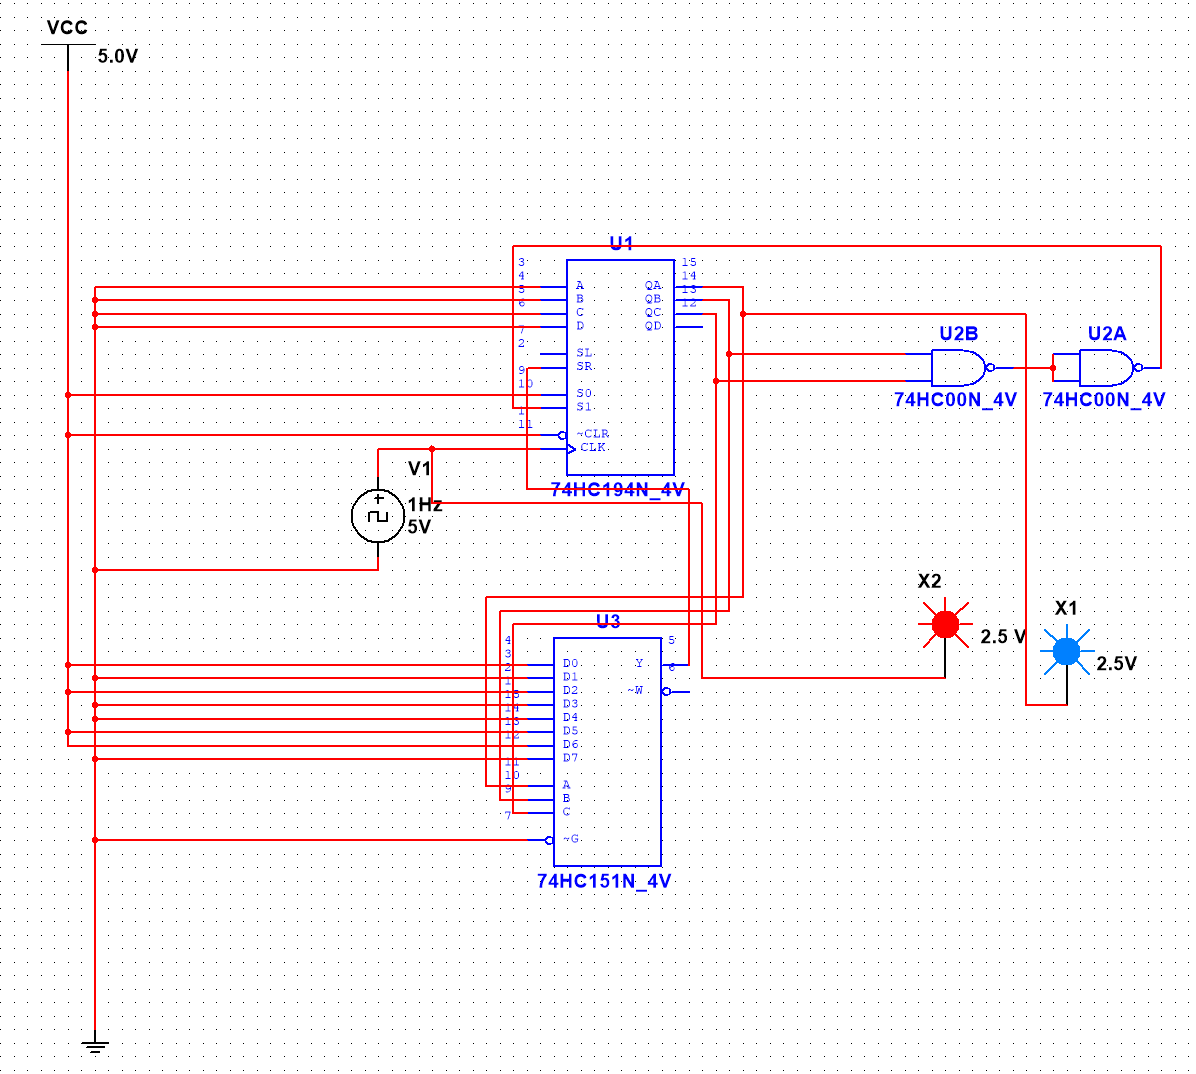
\includegraphics[width=0.6\textwidth]{../img/Ex2_194.png} % 确保文件名和路径正确
    \caption{方案二逻辑电路图}
    \label{fig:SR}
  \end{figure}
\section{测试方案}
\begin{enumerate}
\item 搭接电路,以面包板上自带的时钟脉冲作为时钟信号,把输出端接入LED灯,同时将时钟信号也接入LED灯作为对照,灯亮表示1,灯灭表示0,观察并记录输出序列。
\item 加入TTL连续脉冲,用示波器观察$\mathrm{CLK} $、$\mathrm{Q_0}$、$\mathrm{Q_1}$、$\mathrm{Q_2}$及输出端LED的波形,汇总并记录。
\end{enumerate}
\end{document}